\documentclass[tikz,svgnames,border=0 2]{standalone}

\usepackage{mathtools}

\usetikzlibrary{positioning,arrows,fit}

\renewcommand\vec[1]{\boldsymbol{#1}}

\begin{document}
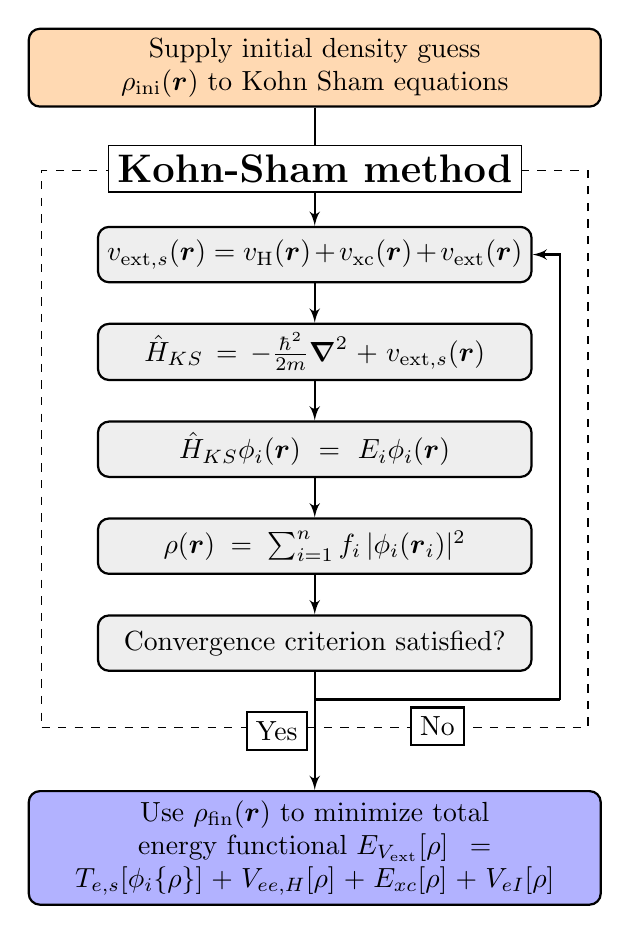
\begin{tikzpicture}[
    box/.style={rectangle,draw,fill=DarkGray!20,node distance=1cm,text width=15em,text centered,rounded corners,minimum height=2em,thick},
    arrow/.style={draw,-latex',thick},
  ]

  \node [box] (potential) {$v_{\text{ext},s}(\vec r)=v_\text{H}(\vec r) + v_\text{xc}(\vec r) + v_\text{ext}(\vec r)$};
  \node [box,below=0.5 of potential] (hamiltonian) {$\hat{H}_{KS}=-\frac{\hbar^2}{2m}\vec{\nabla}^2 + v_{\text{ext},s}(\vec r)$};
  \node [box,below=0.5 of hamiltonian] (se) {$\hat{H}_{KS} \phi_i(\vec r)= E_i \phi_i(\vec r)$};
  \node [box,below=0.5 of se] (density) {$\rho(\vec r)=\sum_{i=1}^n f_i\,|\phi_i(\vec r_i)|^2$};
  \node [box,below=0.5 of density] (criterion) {Convergence criterion satisfied?};

  \path
  (potential.north west) ++(-1em,1em) coordinate (potential fit)
  (criterion.south east) ++(1em,-1em) coordinate (criterion fit);

  \node [box,above=1.5 of potential, fill=orange!30, text width=20em] (initial) {Supply initial density guess $\rho_\text{ini}(\vec r)$ to Kohn Sham equations};
  \node [box,below=1.5 of criterion, fill=blue!30, text width=20em] (energy) {Use $\rho_\text{fin}(\vec r)$ to minimize total energy functional $E_{V_\text{ext}}[\rho]=T_{e,s}[\phi_i\{\rho\}] + V_{ee,H}[\rho] + E_{xc}[\rho] + V_{eI}[\rho]$};

  \path [arrow] (initial) -- (potential);
  \path [arrow] (potential) -- (hamiltonian);
  \path [arrow] (hamiltonian) -- (se);
  \path [arrow] (se) -- (density);
  \path [arrow] (density) -- (criterion);

  \node [rectangle,draw,dashed,inner sep=1em,fit=(potential fit) (criterion fit)] (enclosure) {};
  \node [above=-0.8em of enclosure,anchor=south,draw,outer sep=0pt,fill=white] (enclosure label) {\Large\textbf{Kohn-Sham method}};

  \path [arrow] (criterion) -- (energy) node [midway,left=0.1,draw,outer sep=0pt,fill=white] (TextNode) {Yes};
  \path [draw,thick] (criterion.south) ++(0em,-1em) -- (criterion fit) node [midway,below=0.1,sloped,draw,outer sep=0pt,fill=white] (TextNode) {No};
  \draw [arrow] (criterion fit) |- (potential.east);

\end{tikzpicture}
\end{document}